\section{Mercer谱表示}
\label{sec:rkhs-mercer}

到目前为止，RKHS的全部结构都只由核决定，没有用到测度。本节在定义域上加入一个参考测度，用核作积分核得到积分算子，再借助紧自伴算子的谱理论，把核写成特征函数的展开。这个展开给出RKHS的一组标准正交坐标，也给出一种由核本身确定的有限特征：保留前若干个谱方向。

全节使用下面的标准条件：$X$是紧度量空间，$K$是$X\times X$上连续的正定核，$\mu$是$X$上的有限正Borel测度，并且具有\term{全支撑}（full support），即$X$的每个非空开集测度为正。记$\kappa^2=\max_{x\in X}K(x,x)$，它有限，因为连续函数在紧集上有最大值。

\subsection{核积分算子}
\label{sec:rkhs-integral-operator}

在上述条件下定义\term{核积分算子}（kernel integral operator）
\[
(T_Kf)(x)=\int_XK(x,y)\,f(y)\,\mathrm d\mu(y),\qquad f\in L^2(\mu).
\]
$L^2(\mu)$取内积$\langle f,g\rangle_{L^2}=\int_X\overline f\,g\,\mathrm d\mu$。下面依次核验$T_K$的紧性、自伴性与正性，它们是使用谱定理所需的全部条件。

\paragraph{紧性、自伴性与像的连续性}

$K$连续且$X$紧，所以$\lvert K\rvert\leq\kappa^2$有界，又$\mu$有限，于是$K\in L^2(\mu\otimes\mu)$。第~\ref{chap:linear-operators}章说明，平方可积核给出的积分算子是Hilbert--Schmidt算子，因而是紧算子；由$K(y,x)=\overline{K(x,y)}$，交换积分次序得$\langle g,T_Kf\rangle_{L^2}=\langle T_Kg,f\rangle_{L^2}$，所以$T_K$自伴。

$T_K$的像比一般的$L^2$等价类好得多：对任意$g\in L^2(\mu)$，$T_Kg$是处处有定义的连续函数。事实上，由Cauchy--Schwarz不等式，
\[
\lvert(T_Kg)(x)-(T_Kg)(x')\rvert\leq\mu(X)^{1/2}\sup_{y\in X}\lvert K(x,y)-K(x',y)\rvert\,\lVert g\rVert_{L^2},
\]
而$K$在紧集$X\times X$上一致连续，右端随$x'\to x$趋于零。

\paragraph{积分算子的正性}

自伴只说明$\langle f,T_Kf\rangle$是实数，不说明它非负。正性来自核的正定性，但二者的联系需要一个逼近论证：正定性只涉及有限点组，积分则是连续的累计。

\begin{lemma}[正定连续核给出正算子]
\label{lem:rkhs-positive-operator}
在本节条件下，对一切$f\in L^2(\mu)$，
\[
\langle f,T_Kf\rangle_{L^2}=\iint_{X\times X}\overline{f(x)}\,K(x,y)\,f(y)\,\mathrm d\mu(x)\,\mathrm d\mu(y)\geq0 .
\]
\end{lemma}

\begin{proof}
先设$f$连续。给定$\varepsilon>0$，函数$(x,y)\mapsto\overline{f(x)}K(x,y)f(y)$在紧集上一致连续，取$\delta>0$使两点距离小于$\delta$时它的变化小于$\varepsilon$。用有限个半径$\delta/2$的开球覆盖$X$，再依次去掉重叠部分，得到$X$的有限Borel划分$A_1,\ldots,A_N$，每块直径小于$\delta$；在每块中任取一点$x_i$，令$c_i=f(x_i)\mu(A_i)$。在$A_i\times A_j$上用常数$\overline{f(x_i)}K(x_i,x_j)f(x_j)$代替被积函数，得
\[
\Bigl\lvert\langle f,T_Kf\rangle-\sum_{i,j}\overline{c_i}\,c_j\,K(x_i,x_j)\Bigr\rvert\leq\varepsilon\,\mu(X)^2 .
\]
中间的和是点组$x_1,\ldots,x_N$上Gram矩阵的二次型，非负；令$\varepsilon\to0$即得$\langle f,T_Kf\rangle\geq0$。

对一般的$f\in L^2(\mu)$，连续函数在$L^2(\mu)$中稠密（紧度量空间上的有限Borel测度，见第~\ref{chap:function-approximation}章），而$f\mapsto\langle f,T_Kf\rangle$在$L^2$中连续，非负性保持到极限。
\end{proof}

\paragraph{再生关系与积分算子的区别}

核在这里扮演两种角色，不应混淆。在再生关系$f(x)=\langle K_x,f\rangle_H$中，核截面读取的是$f$在单个点的值，内积是$H$的内积，不涉及任何测度。在积分算子中，$K$对整条函数作加权累计，结果依赖于参考测度：同一个核配上不同的$\mu$，得到不同的算子。

以仿射核$K(x,y)=1+xy$为例，取$X=[-1,1]$。在$\mathrm d\mu=\mathrm dx/2$下，
\[
T_K1=\int_{-1}^1(1+xy)\,\frac{\mathrm dy}{2}=1,\qquad
T_Kx=\int_{-1}^1(1+xy)\,y\,\frac{\mathrm dy}{2}=\frac x3 ,
\]
与$1$、$x$都正交的函数被映为零。若改用$\mathrm d\mu=\mathrm dx$，算子整体变为原来的两倍。核没有变，算子随测度改变。

\subsection{核的谱展开}
\label{sec:rkhs-spectral-expansion}

至此，$T_K$是复Hilbert空间$L^2(\mu)$上的紧、自伴、正算子。第~\ref{chap:operator-spectra}章的谱定理给出：非零特征值都是正数，至多可数，按重数重复排列为$\lambda_1\geq\lambda_2\geq\cdots>0$，只能在零处聚集；相应的标准正交特征函数$\phi_j$构成$(\ker T_K)^\perp$的标准正交基，并且$T_Kf=\sum_j\lambda_j\langle\phi_j,f\rangle_{L^2}\phi_j$在$L^2$范数下成立。特征函数的个数可以有限，也可以无限。

\paragraph{特征函数的连续代表}

特征函数起初只是$L^2$等价类。若$T_K\phi=\lambda\phi$且$\lambda>0$，则$\phi=\lambda^{-1}T_K\phi$几乎处处成立，右端是连续函数，所以$\phi$有连续代表，以下总取这个代表。全支撑保证这个代表唯一：两个连续函数若几乎处处相等，使它们不相等的点组成开集，测度为零，由全支撑只能是空集。

若$\mu$没有全支撑，例如$X=[0,1]$而$\mu$只是$[0,\tfrac12]$上的Lebesgue测度，那么在$(\tfrac12,1]$上任意改动的函数仍是同一个$L^2$元素，积分算子的特征函数无法确定函数在测度支撑之外的取值，下面的逐点展开也就无从谈起。

\paragraph{Mercer定理}

一般紧自伴算子的谱定理只给出算子作用在$L^2$范数下的展开，第~\ref{chap:operator-spectra}章也指出，由此得到的核展开只在乘积空间的$L^2$意义下收敛。在本节的条件下，可以得到核本身的逐点、一致展开，这就是\term{Mercer定理}（Mercer theorem）\scite{mercer1909functions}。

\begin{theorem}[Mercer定理]
\label{thm:rkhs-mercer}
设$X$是紧度量空间，$K$是$X\times X$上连续的正定核，$\mu$是$X$上全支撑的有限正Borel测度。设$\lambda_j>0$与连续的$\phi_j$是$T_K$的全部正特征值与$L^2(\mu)$标准正交特征函数。则
\begin{equation}
K(x,y)=\sum_j\lambda_j\,\phi_j(x)\,\overline{\phi_j(y)}\qquad(x,y\in X),
\label{eq:rkhs-mercer}
\end{equation}
级数在$X\times X$上绝对且一致收敛；并且$\sum_j\lambda_j=\int_XK(x,x)\,\mathrm d\mu(x)<\infty$。
\end{theorem}

\begin{proof}
第一步，对角线上的部分和有界。令$K^{(m)}(x,y)=K(x,y)-\sum_{j\leq m}\lambda_j\phi_j(x)\overline{\phi_j(y)}$，它连续，对应的积分算子满足$\langle f,T^{(m)}f\rangle=\sum_{j>m}\lambda_j\lvert\langle\phi_j,f\rangle\rvert^2\geq0$。若某点$K^{(m)}(x_0,x_0)<0$（对角值是实数），由连续性存在$x_0$的开邻域$U$使$\operatorname{Re}K^{(m)}<0$在$U\times U$上成立。取$f=\mathbf 1_U$，全支撑给出$\mu(U)>0$，于是实数$\langle f,T^{(m)}f\rangle=\iint_{U\times U}\operatorname{Re}K^{(m)}<0$，矛盾。所以对一切$m$与$x$，
\[
\sum_{j\leq m}\lambda_j\lvert\phi_j(x)\rvert^2\leq K(x,x)\leq\kappa^2 .
\]

第二步，固定$x$识别极限。由Cauchy--Schwarz不等式与第一步，
\[
\sum_{j=p}^q\lambda_j\lvert\phi_j(y)\phi_j(x)\rvert\leq\Bigl(\sum_{j=p}^q\lambda_j\lvert\phi_j(x)\rvert^2\Bigr)^{1/2}\kappa ,
\]
右端括号中的级数收敛，所以$S(y,x)=\sum_j\lambda_j\phi_j(y)\overline{\phi_j(x)}$关于$y$一致收敛，$S(\cdot,x)$连续。另一方面，$\langle\phi_j,K(\cdot,x)\rangle_{L^2}=\overline{(T_K\phi_j)(x)}=\lambda_j\overline{\phi_j(x)}$，与$S(\cdot,x)$的系数相同。所以连续函数$h=K(\cdot,x)-S(\cdot,x)$与每个$\phi_j$正交，属于$\ker T_K$；$T_Kh$连续且几乎处处为零，由全支撑处处为零，从而$\int\overline{h}\,K(\cdot,x)\,\mathrm d\mu=\overline{(T_Kh)(x)}=0$。又$\int\overline h\,S(\cdot,x)\,\mathrm d\mu=\sum_j\lambda_j\overline{\phi_j(x)}\langle h,\phi_j\rangle=0$，两式相减得$\int\lvert h\rvert^2\,\mathrm d\mu=0$。由全支撑与连续性，$h\equiv0$，即式~\eqref{eq:rkhs-mercer}逐点成立。

第三步，一致收敛。在对角线上，连续函数$R_m(x)=K(x,x)-\sum_{j\leq m}\lambda_j\lvert\phi_j(x)\rvert^2$随$m$单调下降并逐点趋于零。对任意$\varepsilon>0$，闭集$\{R_m\geq\varepsilon\}$随$m$递减且交为空集，由$X$的紧性，其中某一个已是空集，所以$R_m\to0$一致成立（这就是Dini定理的论证）。再由第二步的Cauchy--Schwarz估计，$\sum_{j>m}\lambda_j\lvert\phi_j(x)\phi_j(y)\rvert\leq\sqrt{R_m(x)R_m(y)}\leq\max R_m$，得到$X\times X$上的绝对一致收敛。最后对对角线逐项积分（一致收敛且$\mu$有限），$\int K(x,x)\,\mathrm d\mu=\sum_j\lambda_j\int\lvert\phi_j\rvert^2\,\mathrm d\mu=\sum_j\lambda_j$。
\end{proof}

比较两种结论：一般紧自伴算子只有$L^2$意义下的谱展开，特征函数只是等价类；Mercer定理在核连续、正定且测度全支撑的条件下，给出核本身的逐点、一致展开，其中每个$\phi_j$都取连续代表。零特征值方向不出现在展开~\eqref{eq:rkhs-mercer}中，下文任何形如“除以$\lambda_j$”的公式都只在正谱方向上使用。

\paragraph{两个核的谱}

仿射核在$[-1,1]$、$\mathrm dx/2$下，由上一小节的计算，正特征值为$\lambda_1=1$、$\lambda_2=\tfrac13$，标准正交特征函数为$\phi_1=1$、$\phi_2=\sqrt3\,x$。Mercer展开只有两项：$1+\tfrac13\cdot3xy=1+xy$；迹为$1+\tfrac13=\int_{-1}^1(1+x^2)\,\tfrac{\mathrm dx}{2}=\tfrac43$。零空间是与$1,x$正交的全部函数，例如$x^2-\tfrac13$，它是无限维的，却不出现在核的展开中。

最小值核在$[0,1]$、Lebesgue测度下有无穷多个正特征值，而且可以精确算出。对连续的$\phi$，
\[
(T_K\phi)(x)=\int_0^xy\,\phi(y)\,\mathrm dy+x\int_x^1\phi(y)\,\mathrm dy ,
\]
右端两次可微，$(T_K\phi)'(x)=\int_x^1\phi$，$(T_K\phi)''=-\phi$，并且$(T_K\phi)(0)=0$，$(T_K\phi)'(1)=0$。所以$T_K\phi=\lambda\phi$（$\lambda>0$）等价于边值问题$\lambda\phi''=-\phi$，$\phi(0)=0$，$\phi'(1)=0$，其解为$\phi(x)=\sin(\omega x)$，其中$\omega=\lambda^{-1/2}$且$\cos\omega=0$。归一化后
\[
\lambda_j=\frac1{\omega_j^2},\qquad \phi_j(x)=\sqrt2\,\sin(\omega_jx),\qquad \omega_j=\Bigl(j-\frac12\Bigr)\pi,\quad j=1,2,\ldots
\]
同样的推导说明$T_K\phi=0$迫使$\phi=-(T_K\phi)''=0$，零空间平凡，这些$\phi_j$构成$L^2(0,1)$的标准正交基。迹的检验：$\sum_j\lambda_j=\sum_j\tfrac{4}{(2j-1)^2\pi^2}=\tfrac12=\int_0^1x\,\mathrm dx$。

图~\ref{fig:rkhs-mercer-spectrum}画出最小值核的前三个特征函数，并比较三种核的特征值衰减：最小值核按$j^{-2}$衰减，$\sigma=0.5$的高斯核衰减得快得多，仿射核只有两个正特征值。核越光滑，积分算子越强烈地压低高频方向；这里只作为数值观察，不作为一般定理使用。图中的特征函数记作$\psi_j$，即本节的$\phi_j$。

\begin{figure}[!htb]
  \centering
  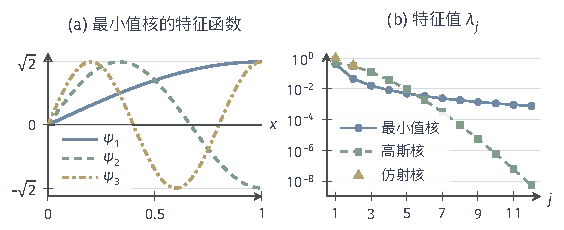
\includegraphics[width=95.5mm]{figures/02-abstract-mathematics/03-function-spaces/tikz/c5-mercer-spectrum/figure.pdf}
  \caption{Mercer特征函数与特征值衰减。(a)~最小值核在$[0,1]$、Lebesgue测度下的前三个特征函数$\psi_j=\sqrt2\sin((j-\frac12)\pi x)$，它们在$0$处为零、在$1$处导数为零；(b)~特征值（对数纵轴）：最小值核$\lambda_j=((j-\frac12)\pi)^{-2}$；高斯核（$\sigma=0.5$，$[-1,1]$，$\mathrm dz/2$）的特征值由40点Gauss--Legendre求积离散计算；仿射核只有$1$与$1/3$两个正特征值。}
  \label{fig:rkhs-mercer-spectrum}
\end{figure}

\subsection{RKHS中的谱坐标}
\label{sec:rkhs-spectral-coordinates}

Mercer展开把核写成了一族加权特征的内积：令$\Phi(x)=\bigl(\sqrt{\lambda_j}\,\overline{\phi_j(x)}\bigr)_j\in\ell^2$，则$\langle\Phi(x),\Phi(y)\rangle_{\ell^2}=\sum_j\lambda_j\phi_j(x)\overline{\phi_j(y)}=K(x,y)$。代入定理~\ref{thm:rkhs-feature-space}，就能读出RKHS在谱坐标下的形式。

\begin{theorem}[RKHS的谱表示]
\label{thm:rkhs-spectral-norm}
在定理~\ref{thm:rkhs-mercer}的条件下：
\begin{enumerate}
\item $\{\sqrt{\lambda_j}\,\phi_j\}$是$H_K$的标准正交基；
\item 函数$f:X\to\mathbb K$属于$H_K$，当且仅当存在数列$(a_j)$满足$\sum_j\lvert a_j\rvert^2/\lambda_j<\infty$，且$f(x)=\sum_ja_j\phi_j(x)$对一切$x$成立。此时级数在$X$上绝对一致收敛，$a_j=\langle\phi_j,f\rangle_{L^2(\mu)}$，并且
\begin{equation}
\lVert f\rVert_{L^2(\mu)}^2=\sum_j\lvert a_j\rvert^2,\qquad \lVert f\rVert_{H_K}^2=\sum_j\frac{\lvert a_j\rvert^2}{\lambda_j}.
\label{eq:rkhs-two-norms}
\end{equation}
\end{enumerate}
\end{theorem}

\begin{proof}
由定理~\ref{thm:rkhs-mercer}，$\lVert\Phi(x)\rVert^2=K(x,x)<\infty$，$\Phi$是$K$的特征映射，对应的函数为$f_w(x)=\langle\Phi(x),w\rangle=\sum_jw_j\sqrt{\lambda_j}\,\phi_j(x)$。先证$\Phi(X)$张成的闭子空间是整个$\ell^2$。设$w\in\ell^2$与每个$\Phi(x)$正交，即$\sum_jw_j\sqrt{\lambda_j}\phi_j(x)=0$对一切$x$成立。系数$w_j\sqrt{\lambda_j}$平方可和，同一级数在$L^2(\mu)$中收敛，其$L^2$极限有一个子列几乎处处收敛到它，所以$L^2$极限为零；由$\phi_j$的标准正交性，$w_j\sqrt{\lambda_j}=0$，即$w=0$。

于是由定理~\ref{thm:rkhs-feature-space}，$w\mapsto f_w$是从$\ell^2$到$H_K$的等距同构，单位向量$e_j$映为$\sqrt{\lambda_j}\phi_j$，这证明第1条。令$a_j=\sqrt{\lambda_j}\,w_j$，条件$w\in\ell^2$就是$\sum_j\lvert a_j\rvert^2/\lambda_j<\infty$，且$\lVert f_w\rVert_{H_K}^2=\sum_j\lvert w_j\rvert^2$。一致收敛来自
\[
\Bigl\lvert\sum_{j>m}a_j\phi_j(x)\Bigr\rvert\leq\Bigl(\sum_{j>m}\frac{\lvert a_j\rvert^2}{\lambda_j}\Bigr)^{1/2}\Bigl(\sum_{j>m}\lambda_j\lvert\phi_j(x)\rvert^2\Bigr)^{1/2}\leq\kappa\Bigl(\sum_{j>m}\frac{\lvert a_j\rvert^2}{\lambda_j}\Bigr)^{1/2} .
\]
一致收敛的级数也在$L^2(\mu)$中收敛到同一函数，由标准正交性得$a_j=\langle\phi_j,f\rangle_{L^2}$与$\lVert f\rVert_{L^2}^2=\sum_j\lvert a_j\rvert^2$。
\end{proof}

\paragraph{两种范数的坐标权重}

式~\eqref{eq:rkhs-two-norms}说明，同一组谱坐标$a_j$在两种范数中得到不同的权重：$L^2$范数对每个坐标一视同仁，RKHS范数把第$j$个坐标的平方放大$1/\lambda_j$倍。$L^2$中的单位方向$\phi_j$在$H_K$中的长度是$\lambda_j^{-1/2}$，$H_K$中真正的单位方向是$\sqrt{\lambda_j}\phi_j$。由于$\lambda_j\to0$，特征值小的方向在RKHS范数中代价很高。

对最小值核，$1/\lambda_j=\omega_j^2$，$\lVert f\rVert_{H_{\min}}^2=\sum_j\omega_j^2\lvert a_j\rvert^2$，这正是$\lVert f'\rVert_{L^2}^2$在余弦基$\sqrt2\cos(\omega_jx)$下的展开。图~\ref{fig:rkhs-norm-weights}中，$f=\phi_1$与$g=\phi_1+0.1\phi_8$的图像几乎重合，$\lVert f-g\rVert_{L^2}=0.1$；但$\lVert f-g\rVert_{H_{\min}}=0.1\,\omega_8=0.75\pi\approx2.36$，比$\lVert f\rVert_{H_{\min}}=\omega_1\approx1.57$还大。高频的小波纹带来很大的导数。

\begin{figure}[!htb]
  \centering
  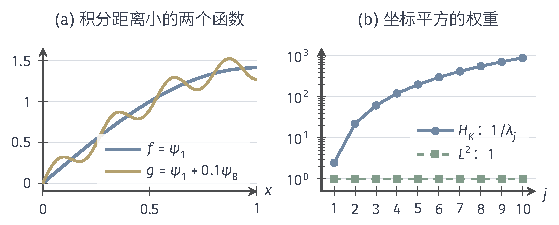
\includegraphics[width=94.6mm]{figures/02-abstract-mathematics/03-function-spaces/tikz/c5-norm-weights/figure.pdf}
  \caption{最小值核下两种范数的谱权重（图中$\psi_j$即正文的$\phi_j$）。(a)~$f=\psi_1$与$g=\psi_1+0.1\psi_8$，$\psi_j=\sqrt2\sin((j-\frac12)\pi x)$；两者的$L^2$距离为$0.1$，核范数距离却约为$2.36$。(b)~谱坐标平方在两种范数中的权重：$L^2$中恒为$1$，$H_K$中为$1/\lambda_j=((j-\frac12)\pi)^2$（对数纵轴），随$j$平方增长。}
  \label{fig:rkhs-norm-weights}
\end{figure}

\paragraph{只使用非零特征方向}

定理~\ref{thm:rkhs-spectral-norm}对$H_K$的成员提出两项要求：作为$L^2$元素，函数没有零特征值方向的分量；谱坐标的加权平方和有限。两项要求可以分别不满足。仿射核下，$x^2=\tfrac13\phi_1+(x^2-\tfrac13)$含有零空间分量$x^2-\tfrac13$，所以不在$H_{\mathrm{aff}}$中。最小值核下零空间平凡，但常数$1$的谱坐标为$a_j=\sqrt2/\omega_j$，$\sum_j\lvert a_j\rvert^2=1$有限，$\sum_j\lvert a_j\rvert^2/\lambda_j=\sum_j2$却发散；常数$1$在$L^2$中有谱展开，却不属于$H_{\min}$，这与$H_{\min}$要求$f(0)=0$相符。

\paragraph{谱坐标依赖测度，RKHS范数不依赖}

仍取仿射核，把$[-1,1]$上的测度从$\mathrm dx/2$换成$\mathrm dx$，特征值变为$2$与$\tfrac23$，标准正交特征函数变为$1/\sqrt2$与$\sqrt{3/2}\,x$。对$f=a+bx$，新的谱坐标为$a_1=\sqrt2\,a$，$a_2=\sqrt{2/3}\,b$，于是
\[
\frac{\lvert a_1\rvert^2}{\lambda_1}+\frac{\lvert a_2\rvert^2}{\lambda_2}=\frac{2a^2}{2}+\frac{2b^2/3}{2/3}=a^2+b^2 ,
\]
与原来的RKHS范数相同；而$L^2$范数平方从$a^2+b^2/3$变成了$2a^2+2b^2/3$。一般地，由定理~\ref{thm:rkhs-moore-aronszajn}，$H_K$的内积只由核决定；测度提供的是一组正交坐标和积分意义下的误差度量。

\subsection{Mercer谱特征的截断}
\label{sec:rkhs-spectral-truncation}

谱坐标给出一种由核与测度共同确定的有限特征：按非增的特征值保留前$N$个非零谱方向$\phi_1,\ldots,\phi_N$，令$V_N=\operatorname{span}\{\phi_1,\ldots,\phi_N\}$，把$f=\sum_ja_j\phi_j$截断为$f_N=\sum_{j\leq N}a_j\phi_j$。因为$\phi_j$在$L^2(\mu)$与$H_K$两种内积下都两两正交，$f_N$同时是$f$在$V_N$上的$L^2$投影与$H_K$投影。

\paragraph{两种尾和}

由式~\eqref{eq:rkhs-two-norms}，两种范数下的截断误差都是系数的尾和，只是权重不同：
\begin{equation}
\lVert f-f_N\rVert_{H_K}^2=\sum_{j>N}\frac{\lvert a_j\rvert^2}{\lambda_j},\qquad
\lVert f-f_N\rVert_{L^2(\mu)}^2=\sum_{j>N}\lvert a_j\rvert^2 .
\label{eq:rkhs-tail-sums}
\end{equation}
若$T_K$只有$r$个非零特征值（有限秩），则$H_K=V_r$是$r$维的，保留全部$r$个非零方向即可精确表示$H_K$中的每个函数，例如仿射核取$N=2$。下面考虑无穷多个非零特征值的情形。

\paragraph{单位球上的$L^2$误差}

对$j>N$有$\lambda_j\leq\lambda_{N+1}$，所以
\begin{equation}
\lVert f-f_N\rVert_{L^2(\mu)}^2=\sum_{j>N}\lambda_j\cdot\frac{\lvert a_j\rvert^2}{\lambda_j}\leq\lambda_{N+1}\lVert f-f_N\rVert_{H_K}^2\leq\lambda_{N+1}\lVert f\rVert_{H_K}^2 .
\label{eq:rkhs-tail-comparison}
\end{equation}
因此对RKHS单位球中的全部函数，$L^2$平方误差有统一的上界$\lambda_{N+1}$，随$N\to\infty$趋于零。这个界不能改进：$f=\sqrt{\lambda_{N+1}}\phi_{N+1}$的RKHS范数为$1$，$L^2$平方误差恰好是$\lambda_{N+1}$。

这个统一界依赖于两种范数的差别，在RKHS范数下没有对应的结论。仍取$f=\sqrt{\lambda_{N+1}}\phi_{N+1}$，它与$V_N$正交，$\lVert f-f_N\rVert_{H_K}=\lVert f\rVert_{H_K}=1$。所以对每个$N$，单位球中总有函数的RKHS截断误差等于$1$，不能推出单位球在RKHS范数下有统一趋零的截断误差。对单个固定的$f\in H_K$，式~\eqref{eq:rkhs-tail-sums}中的RKHS尾和仍趋于零，只是趋于零的速度取决于$f$本身。

\paragraph{逐点误差与核的截断}

RKHS误差还控制逐点误差。$V_N$的再生核是$K_N(x,y)=\sum_{j\leq N}\lambda_j\phi_j(x)\overline{\phi_j(y)}$，由定理~\ref{thm:rkhs-subspace-error}，
\begin{equation*}
\begin{gathered}
\lvert f(x)-f_N(x)\rvert\leq\sqrt{R_N(x)}\,\lVert f-f_N\rVert_{H_K},\\
R_N(x)=K(x,x)-K_N(x,x)=\sum_{j>N}\lambda_j\lvert\phi_j(x)\rvert^2 .
\end{gathered}
\end{equation*}
由Mercer定理，$R_N$一致趋于零，$\int_XR_N\,\mathrm d\mu=\sum_{j>N}\lambda_j$。所以截断后的核$K_N$在$X\times X$上一致逼近$K$，这是核的近似；某个具体函数的误差还要乘上它自己的RKHS尾和。

\begin{example}[最小值核的三项截断]
\label{ex:rkhs-hmin-truncation}
取$q(x)=4x(1-x)\in H_{\min}$。两次分部积分给出谱坐标$a_j=4\sqrt2\bigl(2\omega_j^{-3}-(-1)^{j+1}\omega_j^{-2}\bigr)$，前三项约为$0.626$、$0.363$、$-0.068$。又$\lVert q\rVert_{L^2}^2=\tfrac{8}{15}$，$\lVert q\rVert_{H_{\min}}^2=\tfrac{16}{3}$，用总和减去前三项，得
\[
\lVert q-q_3\rVert_{L^2}\approx0.068,\qquad \lVert q-q_3\rVert_{H_{\min}}\approx1.07 .
\]
核对式~\eqref{eq:rkhs-tail-comparison}：$0.068^2\approx0.0046\leq\lambda_4\times1.07^2\approx0.0083\times1.15\approx0.0095$。RKHS尾和远大于$L^2$尾和，因为$q'(1)=-4\neq0$，而每个$\phi_j$在$1$处导数为零，谱坐标只按$\omega_j^{-2}$衰减。

与例~\ref{ex:rkhs-hmin-interpolation}比较：三个核截面的折线插值，RKHS误差为$\sqrt{16/27}\approx0.77$，小于三项谱截断的$1.07$。核的积分误差则相反：$\int_0^1R_3\,\mathrm dx=\tfrac12-\sum_{j\leq3}\omega_j^{-2}\approx0.034$，小于三个节点的幂函数平方的积分$\int_0^1P_{Z_3}(x)^2\,\mathrm dx=\tfrac{h}{6}=\tfrac1{18}\approx0.056$（由例~\ref{ex:rkhs-hmin-grid}的公式在每个小区间上积分）。两种三维子空间各有所长，哪一种更好取决于所用的误差度量。
\end{example}

谱截断需要先求解积分算子的特征问题，而测度在实际中常常未知或只能由样本给出。由样本点构造Gram矩阵并作谱分解，得到的是第~\ref{sec:rkhs-section-span-approx}节的核截面子空间及其投影核，而不是这里的$K_N$；二者之间的关系涉及抽样误差，本节的尾和结论不能自动搬到这类数值方法上。
